\documentclass{beamer}
\usetheme{metropolis}
\usepackage[ngerman]{babel} 
\usepackage[T1]{fontenc}
\usepackage[utf8]{inputenc}
\usepackage{ragged2e}
\usepackage{biblatex}
\addbibresource{ref.bib}
\usepackage[absolute,overlay]{textpos}
	\setlength{\TPHorizModule}{1pt}
	\setlength{\TPVertModule}{1pt}

\metroset{
	titleformat=smallcaps,
	block=fill
}

\definecolor{titlebg}{HTML}{DDCECD}
\definecolor{titlecolor}{RGB}{0,0,0}
\definecolor{codebg}{HTML}{23373B}
\definecolor{numberbg}{HTML}{EEE5E5}
\definecolor{languagebg}{HTML}{EEE5E5}
\definecolor{languagetext}{RGB}{0, 0, 0}
\definecolor{mintedtext}{HTML}{F8F8F2}

%% MINTED
\usepackage{minted}
\newmintedfile{javascript}{
	linenos,
	autogobble,
	breaklines=true,
	breaksymbol=,
	breakindent=4mm,
	breakbefore=.,
	breakbeforesymbolpre=,
	breakbeforesymbolpost=,
	baselinestretch=0.8,
	framesep=5mm,
	numbersep=7pt,
	fontsize=\footnotesize,
	style=native
}
\newmintedfile{typescript}{
	linenos,
	autogobble,
	breaklines=true,
	breaksymbol=,
	breakindent=4mm,
	breakbefore=.,
	breakbeforesymbolpre=,
	breakbeforesymbolpost=,
	baselinestretch=0.8,
	framesep=5mm,
	numbersep=7pt,
	fontsize=\footnotesize,
	style=native
}
\newmintedfile{html}{
	linenos,
	autogobble,
	breaklines=true,
	breaksymbol=,
	breakindent=4mm,
	breakbefore=.,
	breakbeforesymbolpre=,
	breakbeforesymbolpost=,
	baselinestretch=0.8,
	framesep=5mm,
	numbersep=7pt,
	fontsize=\footnotesize,
	style=native
}

\renewcommand{\theFancyVerbLine}{\sffamily
	\textcolor[RGB]{32,32,32}{\tiny\textrm{\arabic{FancyVerbLine}}}}

%% Minted background
% https://gist.github.com/mutbuerger/e65575180b99e9074129
\usepackage{tcolorbox}
\tcbuselibrary{skins, breakable}
\usetikzlibrary{shadings, backgrounds}
\newtcolorbox{bpbox}[2][]
{%
	enhanced,
	colbacktitle=titlebg,
	coltitle=titlecolor,
	interior style={%
		top color=codebg,
		bottom color=codebg
	},
	boxrule=0mm,
	arc=0mm,
	width= (\linewidth),
	fonttitle=\footnotesize,
	adjusted title=\texttt{#1},
	after title={%
		\hfill\setlength{\fboxsep}{3.5pt}
		\colorbox{languagebg}{\textcolor{languagetext}
			{\scriptsize{\texttt{\hspace{1pt}#2\hspace{1pt}}}}}
	},
	overlay={%
		\begin{tcbclipinterior}\fill[numberbg] (frame.south west)
			rectangle ([xshift=5mm]frame.north west);
		\end{tcbclipinterior}
	},
	top=0mm,
	bottom=0mm,
	left=5mm,
	right=0mm
}



\title{BombermanVR}
\date{03. Februar 2017}
\author{Filip Krakowski}
\institute{Master-Seminar zu Virtueller \& Erweiterter Realität}
\titlegraphic{
\includegraphics[width=3cm]{bilder/hhu-logo.pdf}}

\begin{document}
  \maketitle
  
  \section{Motivation}
  \begin{frame}{Motivation}
  	\begin{center}
  		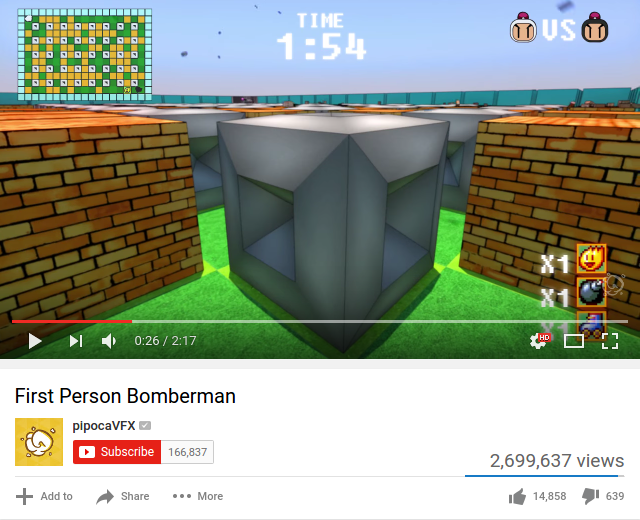
\includegraphics[height=.9\textheight]{bilder/youtube.png}
  	\end{center}
  \end{frame}
  
  
  
%  \begin{frame}{Monolithische Systeme - Deployment}
%  	\begin{center}
%  		Anwendungen können \alert{in einem Schritt} verteilt werden
%  	\end{center}
%  	
%  	\vspace{20pt}
%  	
%  	\includegraphics[width=\textwidth]{bilder/monolith_deployment.pdf}
%  \end{frame}
  
  \begin{frame}{Motivation}
  	\begin{center}
  		
\includegraphics[width=.9\textwidth]{bilder/comment_1.png}
  	\end{center}
  	
  	\begin{center}
  		
\includegraphics[width=.9\textwidth]{bilder/comment_2.png}
  	\end{center}
  	
  	\begin{center}
  		
\includegraphics[width=.9\textwidth]{bilder/comment_3.png}
  	\end{center}
  	
  	\begin{center}
  		
\includegraphics[width=.9\textwidth]{bilder/comment_4.png}
  	\end{center}
  	
  	\begin{center}
  		
\includegraphics[width=.9\textwidth]{bilder/comment_5.png}
  	\end{center}
  	
  	
  	\begin{center}
  		Drei-Schichten-Architektur sehr beliebt
  	\end{center}
  \end{frame}
  
  \section{Anwendung}
  
  \begin{frame}{Software}
  	\begin{center}
  		
\includegraphics[width=.75\textwidth]{bilder/googlevrunity.pdf}
  	\end{center}
  \end{frame}
  
  \begin{frame}{Optimierung}
  	\begin{center}
  		Google VR benötigt zusätzliche Rechenleistung, welche auf vielen mobilen Geräten beschränkt Verfügbar ist. Aus diesem Grund wurden diverse Techniken zur Optimierung angewendet.
  	\end{center}
  \end{frame}
  
  \begin{frame}{Draw Call Batching}
  	\textbf{Dynamic Batching}\\
  	Wird (eingeschränkt) automatisch ausgeführt.
  	\begin{center}
  			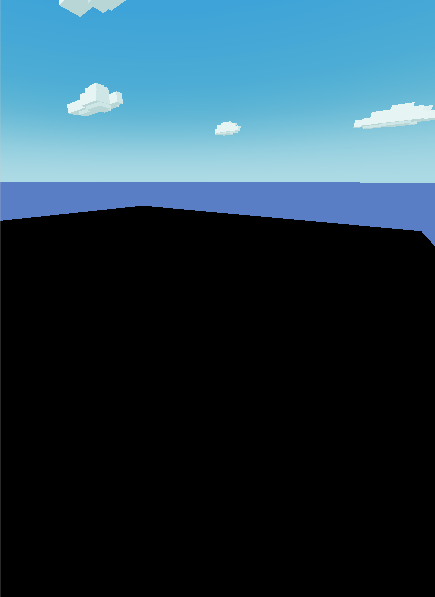
\includegraphics[width=.19\textwidth]{bilder/drawcall/d_1.png} \hfill
  			
\includegraphics[width=.19\textwidth]{bilder/drawcall/d_2.png} \hfill
  			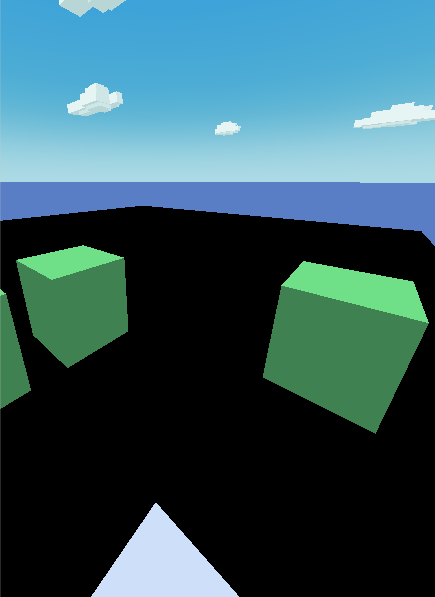
\includegraphics[width=.19\textwidth]{bilder/drawcall/d_3.png} \hfill
  			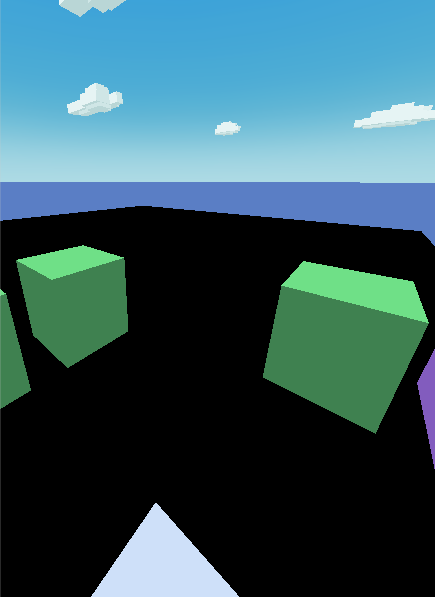
\includegraphics[width=.19\textwidth]{bilder/drawcall/d_4.png} \hfill
  			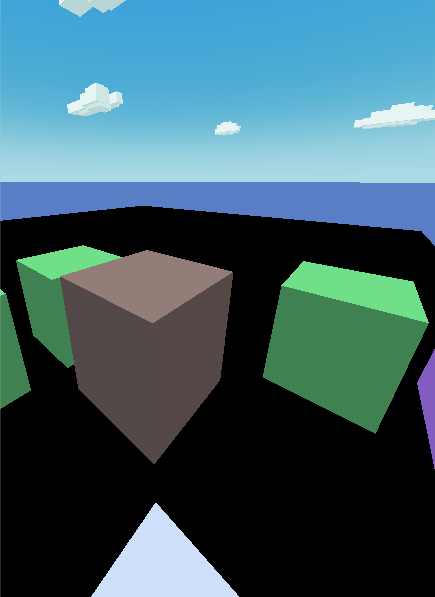
\includegraphics[width=.19\textwidth]{bilder/drawcall/d_5.png}
  	\end{center}
  	
  	\begin{center}
  		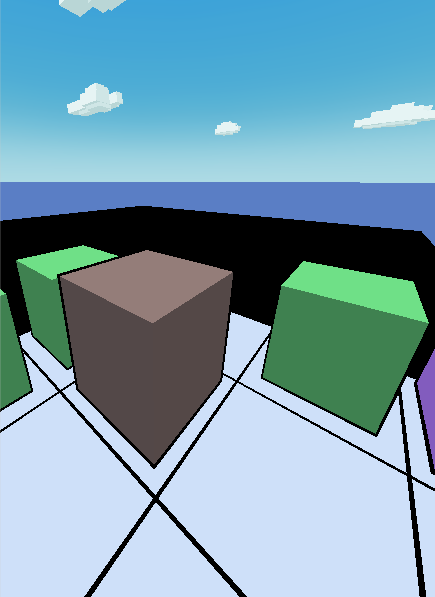
\includegraphics[width=.19\textwidth]{bilder/drawcall/d_6.png} \hfill
  		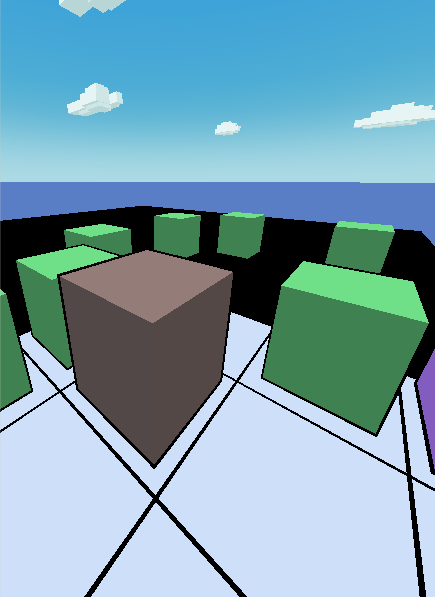
\includegraphics[width=.19\textwidth]{bilder/drawcall/d_7.png} \hfill
  		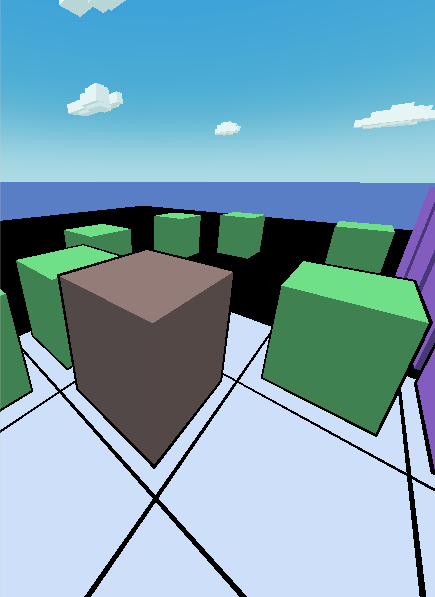
\includegraphics[width=.19\textwidth]{bilder/drawcall/d_8.png} \hfill
  		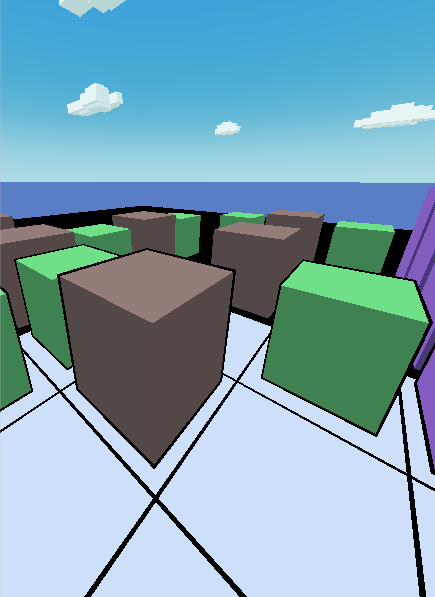
\includegraphics[width=.19\textwidth]{bilder/drawcall/d_9.png} \hfill
  		
\includegraphics[width=.19\textwidth]{bilder/drawcall/d_more.png}
  	\end{center}
  \end{frame}
  
  \begin{frame}{Draw Call Batching}
  	\textbf{Static Batching}\\
  	Muss manuell aktiviert werden.
  	\begin{center}
  		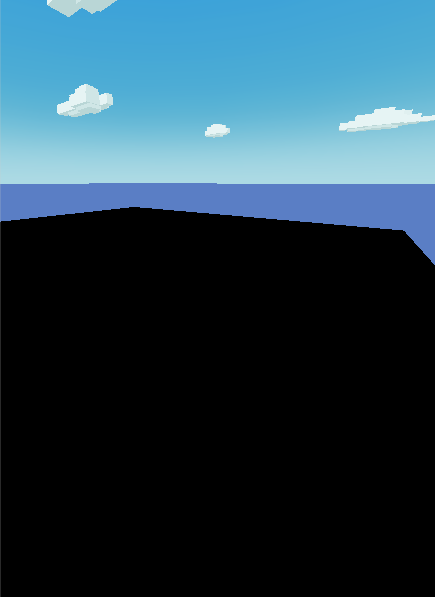
\includegraphics[width=.19\textwidth]{bilder/drawcall/s_1.png} \hfill
  		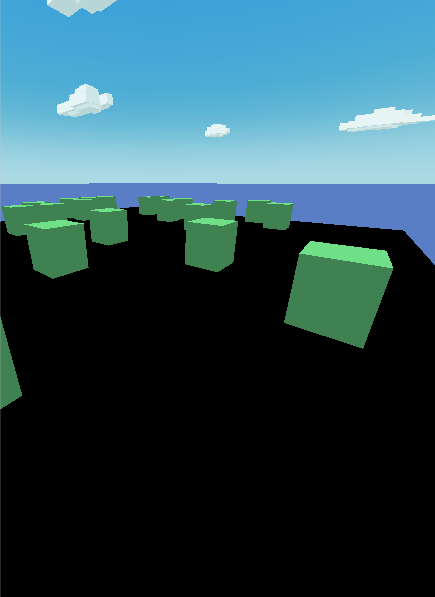
\includegraphics[width=.19\textwidth]{bilder/drawcall/s_2.png} \hfill
  		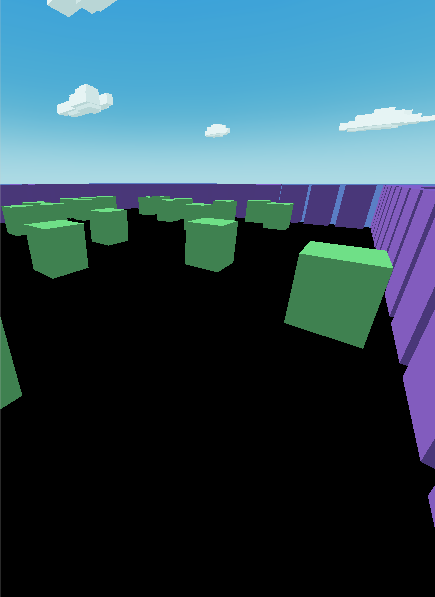
\includegraphics[width=.19\textwidth]{bilder/drawcall/s_3.png} \hfill
  		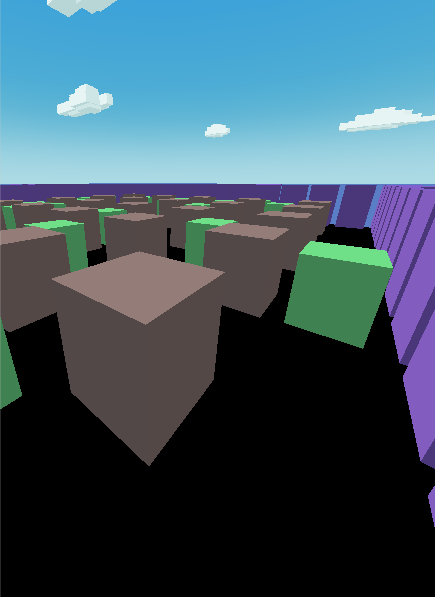
\includegraphics[width=.19\textwidth]{bilder/drawcall/s_4.png} \hfill
  		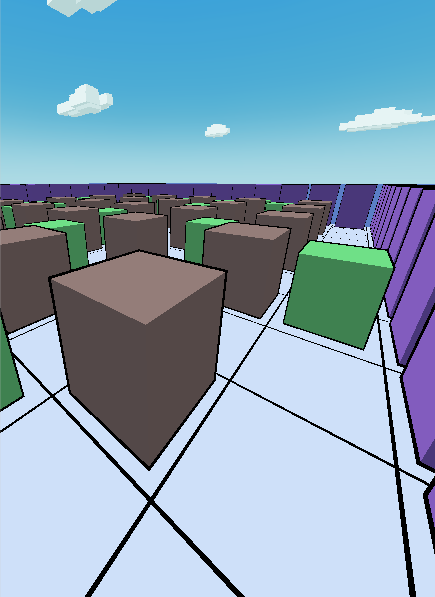
\includegraphics[width=.19\textwidth]{bilder/drawcall/s_5.png}
  	\end{center}
  	
	\justify
  	{\large ``In order to take advantage of static batching, you need to explicitly specify that certain GameObjects are static and do not move, rotate or scale in the game. To do so, mark GameObjects as static using the \textbf{Static} checkbox in the Inspector''}\\
  	\vspace{1pt}
  	\hspace*\fill{\small--- Unity Online Documentation}
  	
  \end{frame}
  
  \begin{frame}{Draw Call Batching}
	\begin{center}
		{\Large
		Was die Dokumentation leider nicht verrät:}\\
		\vspace{10pt}
		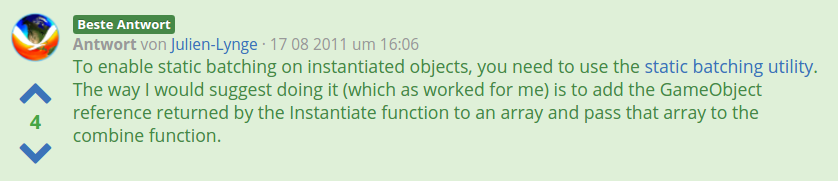
\includegraphics[width=\textwidth]{bilder/staticanswer.png}
	\end{center}
	
	{\Large \textbf{StaticBatchingUtility.Combine}}\\
	public static void \textbf{Combine}(GameObject \textbf{staticBatchRoot})\\
	
	\vspace{-15pt}
	
	StaticBatchingUtility.Combine prepares all children of the \texttt{staticBatchRoot} for static batching. Once combined, children cannot change their \texttt{Transform} properties; however, staticBatchRoot can be moved.
  \end{frame}

  
  \begin{frame}{(Networked) Object Pooling}
  	\begin{center}
  		Oft werden häufig genutzte Objekte ``Just-in-time''\\ instanziiert und hinterher wieder zerstört.
  	\end{center}
  	\begin{center}
  		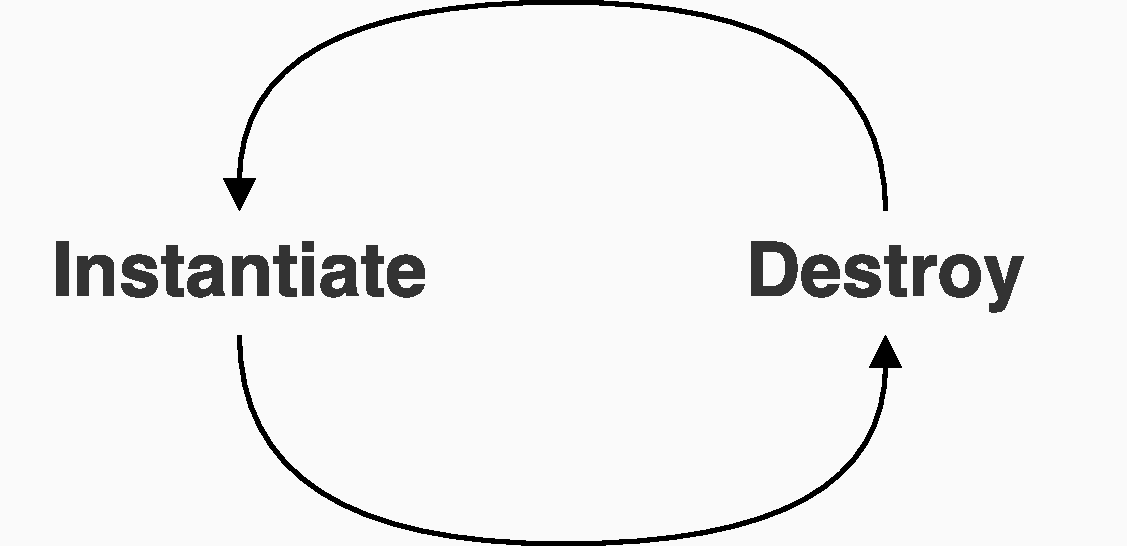
\includegraphics[width=.6\textwidth]{bilder/instantiate.pdf}
  	\end{center}
  	\begin{center}
  		Hochfrequente Instanziierung kostet!\\Garbage Collector wird unnötig belastet!
  	\end{center}
  \end{frame}
  
  \begin{frame}{(Networked) Object Pooling}
  	\begin{center}
  		Zu Beginn des Spiels wird ein \emph{Object Pool} erstellt. Dieser instanziiert eine bestimmte Anzahl an Objekten und stellt diese beispielsweise über eine Queue zur Verfügung.
  	\end{center}
  	\begin{center}
  		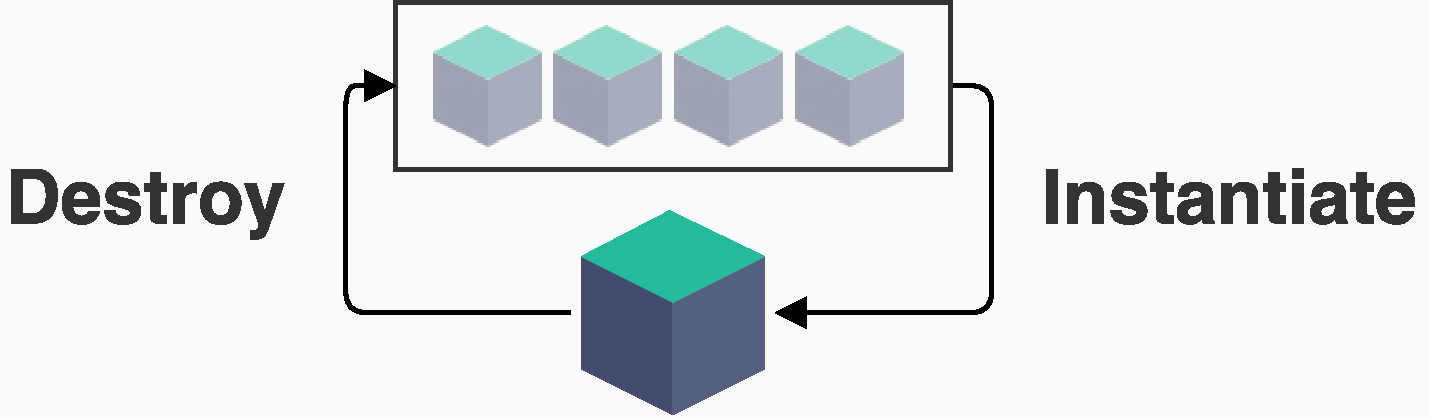
\includegraphics[width=.9\textwidth]{bilder/objectpool.pdf}
  	\end{center}
  	\begin{center}
  		Objekte können wiederbenutzt werden.\\Garbage Collector wird entlastet.
  	\end{center}
  \end{frame}
  
  \begin{frame}{(Networked) Object Pooling}
  	\begin{center}
  		Standardmäßig werden Objekte auf dem Client normal\\ instanziiert nachdem der Server die Anweisung gibt. Dieses Verhalten kann mittels eigener \emph{SpawnHandler} verändert werden. 
  	\end{center}
  	\begin{center}
  		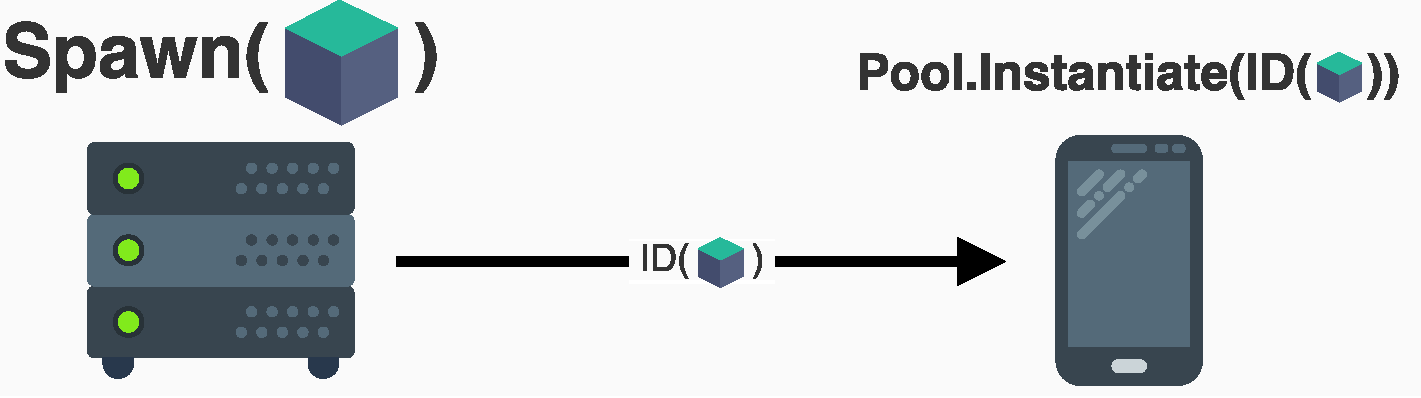
\includegraphics[width=.9\textwidth]{bilder/networkpool.pdf}
  	\end{center}
  	\begin{center}
  		Clients erhalten die ID des zu erstellenden Objekts und nutzen eine Instanz aus dem Pool (anstatt Instanziierung).
  	\end{center}
  \end{frame}
  
  \begin{frame}{Multiplayer}
  	\begin{center}
  		Um Port Forwarding und Ähnliches zu vermeiden \\werden Unitys \emph{Relay Server} verwendet. \\Bis zu 20 Spieler gleichzeitig mit je 4608 B/s kostenlos.
  	\end{center}
  	\begin{center}
  		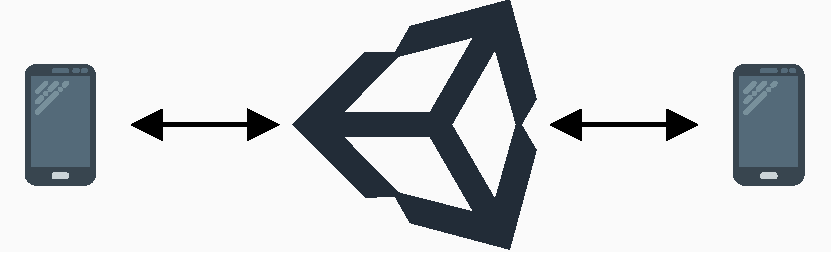
\includegraphics[width=.9\textwidth]{bilder/relay.pdf}
  	\end{center}
  	\begin{center}
  		Alle Clients und Server halten eine Verbindung zum Relay-Server, welcher Nachrichten zwischen ihnen austauscht.\\
  	\end{center}
  \end{frame}
  
  
  
%    \section{Self-Contained Systems}
%    \begin{frame}{Self-Contained Systems - Architektur}
%    	\begin{center}
%    		Mehrere \emph{Self-Contained Systems} bilden im\\ Zusammenspiel ein großes vollständiges System
%    	\end{center}
%    	\vspace{-5pt}
%    	\includegraphics[width=\textwidth]{bilder/scs.pdf}
%    	\vspace{-10pt}
%    	\begin{center}
%    		Jedes Self-Contained System liefert sein \alert{eigenes} Frontend
%    	\end{center}
%    \end{frame}
%    
%    \begin{frame}{Self-Contained Systems - Integration}
%    	\begin{center}
%    		Die Integration eines Self-Contained Systems kann\\ beispielsweise mit Hilfe von \emph{Web Components} erfolgen
%    		
%    		\begin{bpbox}[index.html]{HTML}
%    			\htmlfile[firstline=2]{code/imports/index.html}
%    		\end{bpbox}
%    		
%    		Weboberfläche bildet sich aus \alert{unabhängigen} Fragmenten
%    	\end{center}
%    \end{frame}
  
  
  \begin{frame}[standout]
  	Demo!
  \end{frame}
  
  \begin{frame}{Quellen - Icons}
  	\begin{center}
  		
\includegraphics[width=.5\textwidth]{bilder/flaticon.pdf}
  		
  		\vspace{-40pt}
  		
  		Icons designed by \href{http://www.flaticon.com/authors/madebyoliver}{madebyoliver} from Flaticon 
  	\end{center}
  \end{frame}
    
  \begin{frame}[standout]
  	Fragen?
  \end{frame}
  
\end{document}